\subsection{Analysis}
We provide a comprehensive comparison between RCS and existing CS method in \autoref{tab:compare}. Below, we analyze each property in detail.

\begin{table*}
\centering
 \scalebox{0.75}{
    \begin{tabular}{@{}l|cccccc@{}}
    \toprule
\textbf{Algorithm}  & \textbf{Safety} & \textbf{Liveness} & \textbf{Anti-Collusion} & \textbf{Half-Resilience} & \textbf{Termination} &\textbf{Time Complexity}\\
    \midrule
Consensus Sampling & \textcolor{nGreen}{\ding{51}} & \textcolor{nRed}{\ding{55}} & \textcolor{nRed}{\ding{55}} & \textcolor{nRed}{\ding{55}} & \textcolor{nGreen}{\ding{51}} & $\mathcal{O}(RI)$\\
Reliable Consensus Sampling & \textcolor{nGreen}{\ding{51}} & \textcolor{nGreen}{\ding{51}} & \textcolor{nGreen}{\ding{51}} & \textcolor{nGreen}{\ding{51}} & \textcolor{nGreen}{\ding{51}} & $[\mathcal{O}(RI), \ \mathcal{O}(RI + n^2 \log n)]$\\
    \bottomrule
    \end{tabular}
 }
 \caption{A comprehensive comparison between our proposed RCS and existing method.}
    \label{tab:compare}
\end{table*}


\noindent
\textbf{Latency}. Let $I$ denote the time required to sample $y$ from a distribution $p_i$.
In RCS, if no sample is accepted after $R$ rounds, the algorithm incurs an additional cost of $n^2 \log n$ for trace computation. This cost is negligible compared with $I$, especially for reasoning LLMs \citep{chen2025towards}. Therefore, RCS and CS have comparable time complexity.



\noindent
\textbf{Anti-Collusion}. The goal of collusion is to make $\mathcal{MG}$ more likely to deliver unsafe responses by manipulating one or more Byzantine models. We study the relation between acceptance probabilities of an unsafe response $y_t$ and a safe response $y_v$ within the $R$ round loop of Algorithm \ref{alg:consensus}. We focus on the quantity $\Delta(\sigma) = \sigma(y_t) - \sigma(y_v)$. The detailed derivation appears in \autoref{app:ac}. The sign of $\Delta(\sigma)$ depends on:
\[
\mathcal{D}_{t,v} =
\frac{
\sum_{i = 1}^{s} p_{(i)}(y_t) \sum_{i = s+1}^{n} p_{(i)}(y_v)
}{
\sum_{i = 1}^{s} p_{(i)}(y_v) \sum_{i = s+1}^{n} p_{(i)}(y_t)
}.
\]

When the Byzantine model assigns a very low probability to $y_v$, the value of
$\sum_{i=1}^{s} p_{(i)}(y_v)$ decreases, leading to $\mathcal{D}_{t,v} > 1$. As a result, $\Delta(\sigma) > 0$, which significantly increases the acceptance probability of the unsafe response $y_t$ relative to $y_v$. This effect weakens the security of $\mathcal{MG}$. When unsafe models collude, we present the resulting model probability distributions in \autoref{fig:distribution}. The adversarial behavior of unsafe models clearly has a significant impact on the probability overlap among models in CS. In contrast, the design in lines 9-12 of Algorithm \ref{alg:consensus} effectively mitigates this issue. When the values of $p_{\text{unsafe}}(y_v)_j$ are very low, RCS can significantly downweight their influence on the final output response.



\begin{figure*}[!]
    \centering
    \begin{subfigure}{0.48\textwidth}
        \centering
        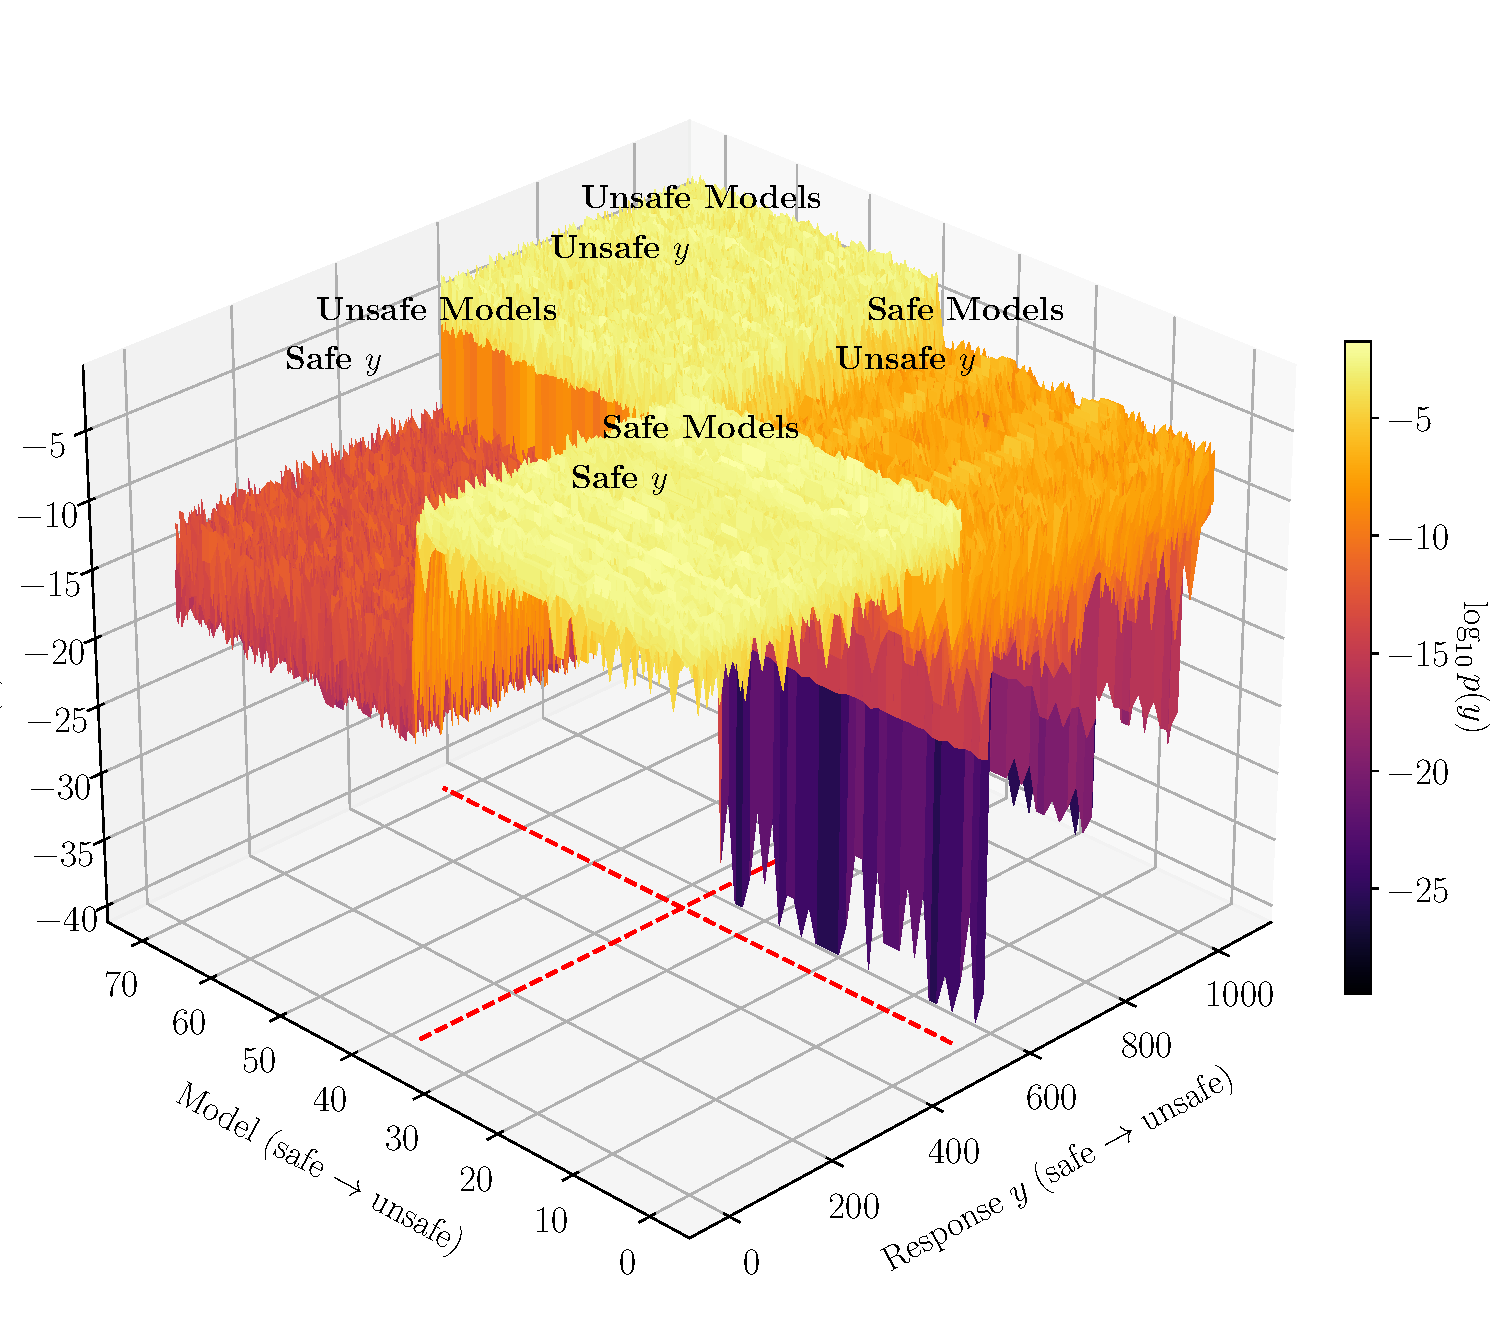
\includegraphics[width=\linewidth]{latex/eval/distribution.pdf}
        \caption{Distribution under general adversarial conditions.}
    \end{subfigure}
    % \hspace{40pt}
    \begin{subfigure}{0.48\textwidth}
        \centering
        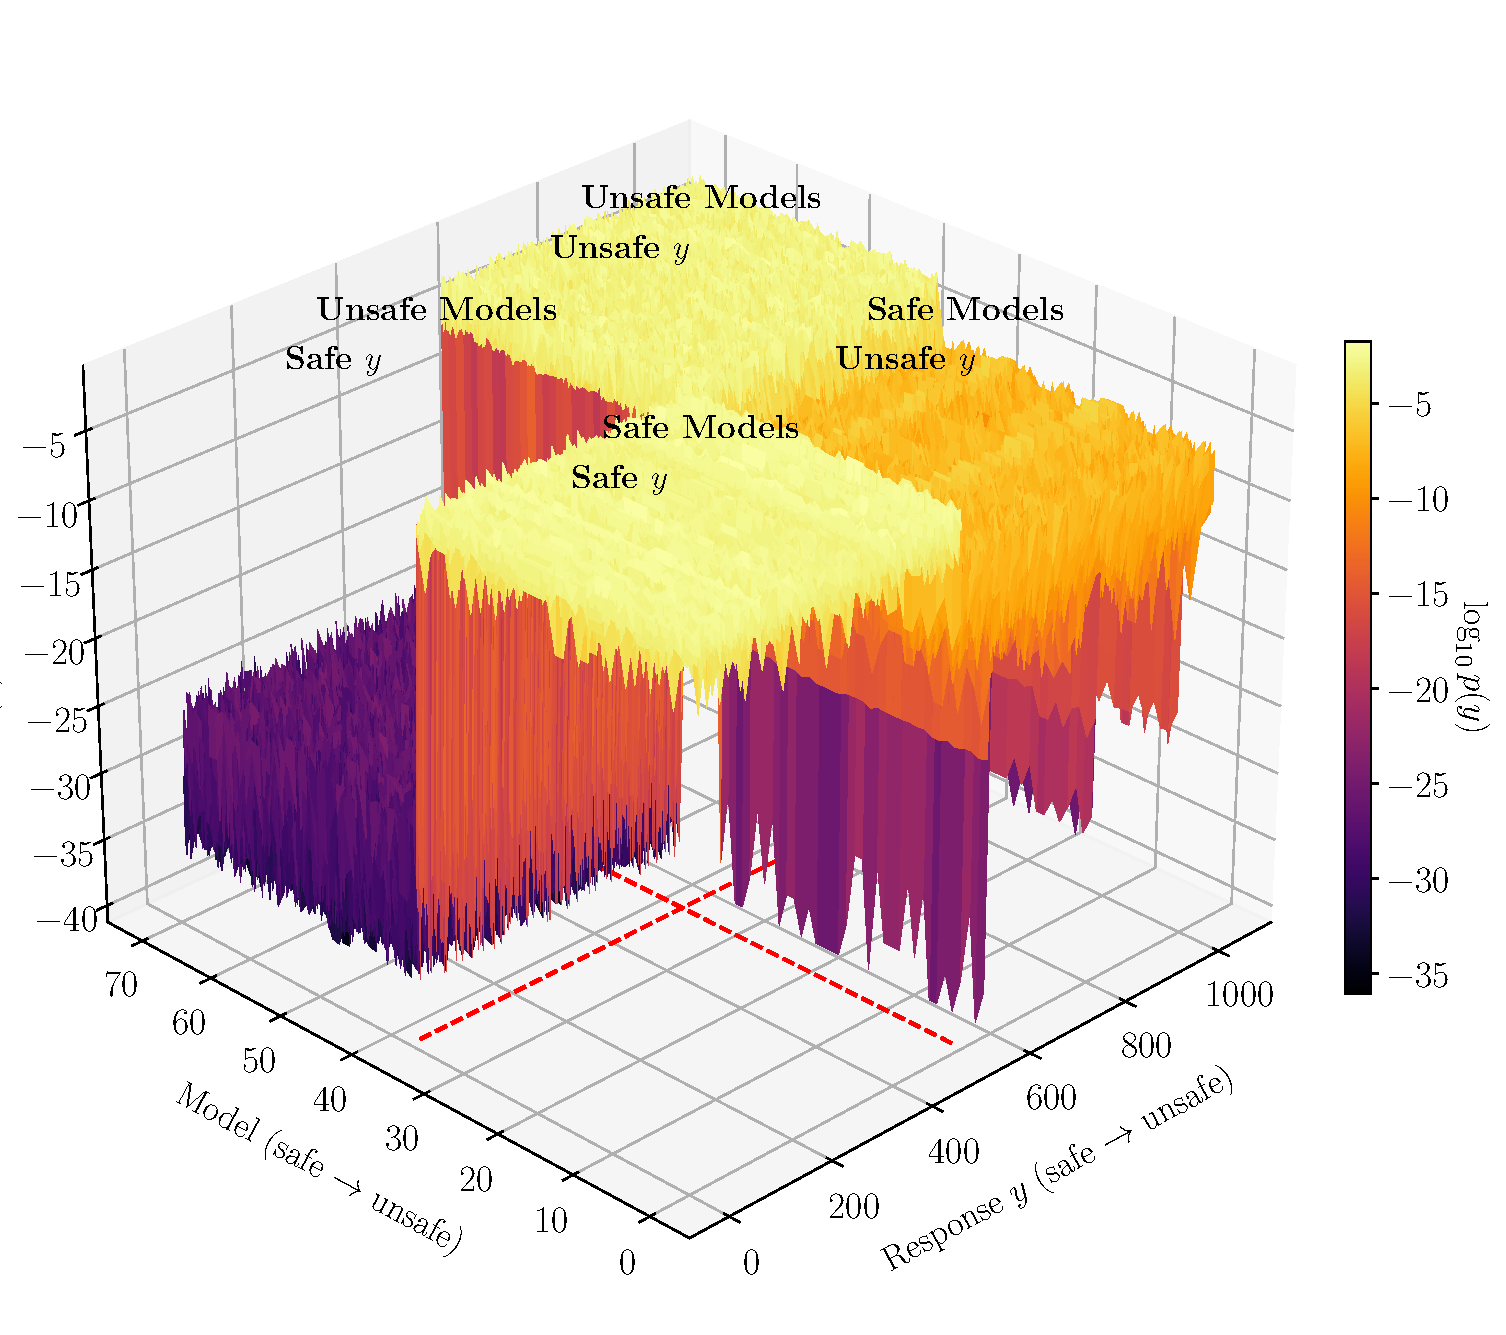
\includegraphics[width=\linewidth]{latex/eval/distribution2.pdf}
        \caption{Distribution under malicious collusion.}
    \end{subfigure}
    \caption{Model probability distribution for consensus sampling under diverse adversarial environments.}
    \label{fig:distribution}
    \vspace{-15pt}
\end{figure*}




\noindent
\textbf{Half-Resilience}. The CS algorithm has an abstention bound, meaning $\Pr[y=\bot]$ does not exceed a threshold when $f < \lceil \frac{n}{2} \rceil$. However, if this condition is violated, the CS abstention bound is affected, leading to an increased probability of abstention and a significant impact on liveness. RCS can avoid this issue. We further validate the half-resilience of RCS in the experiments in Section \ref{sec:experiment}.

\noindent
\textbf{Termination}. 
According to Algorithm \ref{alg:consensus}, for a finite $R$, RCS always terminates within $R$ rounds.



